\chapter{Ergebnisse}\label{chap:Ergebnisse}
Die Vorauslegungwurde mit folgenden Werten durchgeführt:\\
- Isotherm auf: \SI{38}{\celsius}\\
- Avionik Abwärme: \SI{40}{W}\\
- \SI{1}{m} Kontourlänge\\
- Radiator Emissionsgrad: \SI{0,91}{} (AZ-93)\\
- Radiator Absorptionsgrad: \SI{0,15}{} (AZ-93)\\
- Icosane PCM\\
- Trajektoriensimulation\\
- \SI{1}{\frac{kW}{m^2}} mit 50\% dutycycle durch Rotation der Rakete\\
Zu beachten ist, dass die Radiatorleistung konstant bleibt, da das System als isotherm mit einer
infinitesimalen Temperaturerhöhung über den Schmelzpunkt hinweg angenommen wird.\\
Als nächstes sieht man die Flugdaten

\begin{figure}[H]
    \centering

    % Column 1, Row 1
    \begin{subfigure}{0.48\textwidth}
        \centering
        \includegraphics[width=\linewidth]{../../Code/acceleration_over_time.pdf}
        \caption{Beschleunigung während Flug}
        \label{fig:acceleration_over_time}
    \end{subfigure}
    \hfill
    % Column 2, Row 1
    \begin{subfigure}{0.48\textwidth}
        \centering
        \includegraphics[width=\linewidth]{../../Code/altitude_over_time.pdf}
        \caption{Flughöhe}
        \label{fig:altitude_over_time}
    \end{subfigure}

    \vspace{1em}

    % Column 1, Row 2
    \begin{subfigure}{0.48\textwidth}
        \centering
        \includegraphics[width=\linewidth]{../../Code/pressure_over_time.pdf}
        \caption{Statischer Luftdruck während Flug}
        \label{fig:pressure_over_time}
    \end{subfigure}
    \hfill
    % Column 2, Row 2
    \begin{subfigure}{0.48\textwidth}
        \centering
        \includegraphics[width=\linewidth]{../../Code/temperature_over_time.pdf}
        \caption{Statische Lufttemperatur während Flug}
        \label{fig:temperature_over_time}
    \end{subfigure}

    \vspace{1em}

    % Column 1, Row 3
    \begin{subfigure}{0.48\textwidth}
        \centering
        \includegraphics[width=\linewidth]{../../Code/velocity_over_time.pdf}
        \caption{Geschwindigkeit während Flug}
        \label{fig:velocity_over_time}
    \end{subfigure}
    \hfill
    % Column 2, Row 3
    \begin{subfigure}{0.48\textwidth}
        \centering
        \includegraphics[width=\linewidth]{../../Code/dynp_during_flight.pdf}
        \caption{Dynamischer Druck während Flug}
        \label{fig:dynp_over_time}
    \end{subfigure}

\end{figure}

\section{PCM-Radiator-Hybrid}\label{sec:pcmRadiatorHybridErgebnisse}

Als nächstes sieht man Graphen

\begin{figure}[H]
  \centering
  \includegraphics[width=\linewidth]{../../Code/pcm_radiator_hybrid_heatflux_nosim.pdf}\label{fig:pcm_waermestrom_vorauslegung}
  \caption{PCM Wärmestrom während Flug}
  \includegraphics[width=\linewidth]{../../Code/re_pr_during_flight.pdf}\label{fig:re_pr_flugsimulation}
  \caption{Reynolds- und Prandtlzahl während kritischer Phase im Flug}
\end{figure}

\section{Simulationsergebnisse}

\subsection{Aerothermal}

als nächstes habe ich geschaut wo der maximale dynamische Druck erreicht wurde in der Vorauslegung. Die korrespondierenden Werte des Flugzustandes
habe ich dann als Boundery Conditions in der \ac{cfd}~Simulation genommen.
Um zu verifizieren, dass dort auch die maximale Aufheizung stattfindet, habe ich 1 Sekunden vorher und nachder
im Flug die BC's auch verwendet und einen Vergleich gezogen.\\
Maximaler dynamischer Druck: 112901.25708461029 Pa at 28.691 s\\
Entsprechender Flugzustand: 10244.138 m, 750.704 m/s, -51.587°C, 254.783 hPa mit entsprechender Luft Dichte \SI{0.4006}{kg/m^3}\\
Flugzustand bei 18.691 s \ac{maxq} - $\SI{10}{\second}$: 4274.387 m, 461.355 m/s, -12.784, 594.935 hPa mit entsprechender Luft Dichte \SI{0.7960}{kg/m^3}\\
Flugzustand bei 38.691 s \ac{maxq} + $\SI{10}{\second}$: 19758.652 m, 1189.968 m/s, -56.5°C, 56.93 hPa mit entsprechender Luft Dichte \SI{0.0915}{kg/m^3}\\
Flugzustand bei 48.7 s \ac{maxq} + $\SI{20}{\second}$: 32439.616 m, 1393.377 m/s, -43.269°C, 8.136 hPa mit entsprechender Luft Dichte \SI{0.01233001}{kg/m^3}\\
Da wie in~\ref{fig:spezifischer_waermestrom_maxQ_simulationen} zu sehen ist, der Zeitpunkt des maximalen dynamischen Druckes nicht im größten spezifischen
Wärmestrom resultiert, wurde mit der Simulation die den höheren spezifischen Wärmestrom ergeben hat, eine Lösungsfortsetzung durchgeführt um das Maximum zu finden.\\

\begin{figure}[H]
  \centering
  \includegraphics[width=\linewidth]{../../Code/maxQ_compare_heatflux.pdf}
  \caption{Spezifischer Wärmestrom an der Außenhaut bei maximalem dynamischen Druck, sowie \SI{10}{s} davor, danach und \SI{20}{s} danach}\label{fig:spezifischer_waermestrom_maxQ_simulationen}
\end{figure}

\begin{figure}[H]
  \centering
  \includegraphics[width=\linewidth]{../../Code/maxQ_compare_yplus.pdf}
  \caption{y+ Wert an der Außenhaut bei maximalem dynamischen Druck, sowie \SI{10}{s} davor, danach und \SI{20}{s} danach}\label{fig:yplus_maxQ_simulationen}
\end{figure}

\begin{figure}[H]
  \centering
  \includegraphics[width=\linewidth]{../../Code/pcm_radiator_hybrid_heatflux_with_sim.pdf}
  \caption{PCM Wärmestrom während Flug mit Simulationsergebnissen und Fit Kurve}\label{fig:pcm_waermestrom_sim}
\end{figure}

\begin{figure}[H]
    \centering

    \begin{subfigure}{\textwidth}
        \centering
        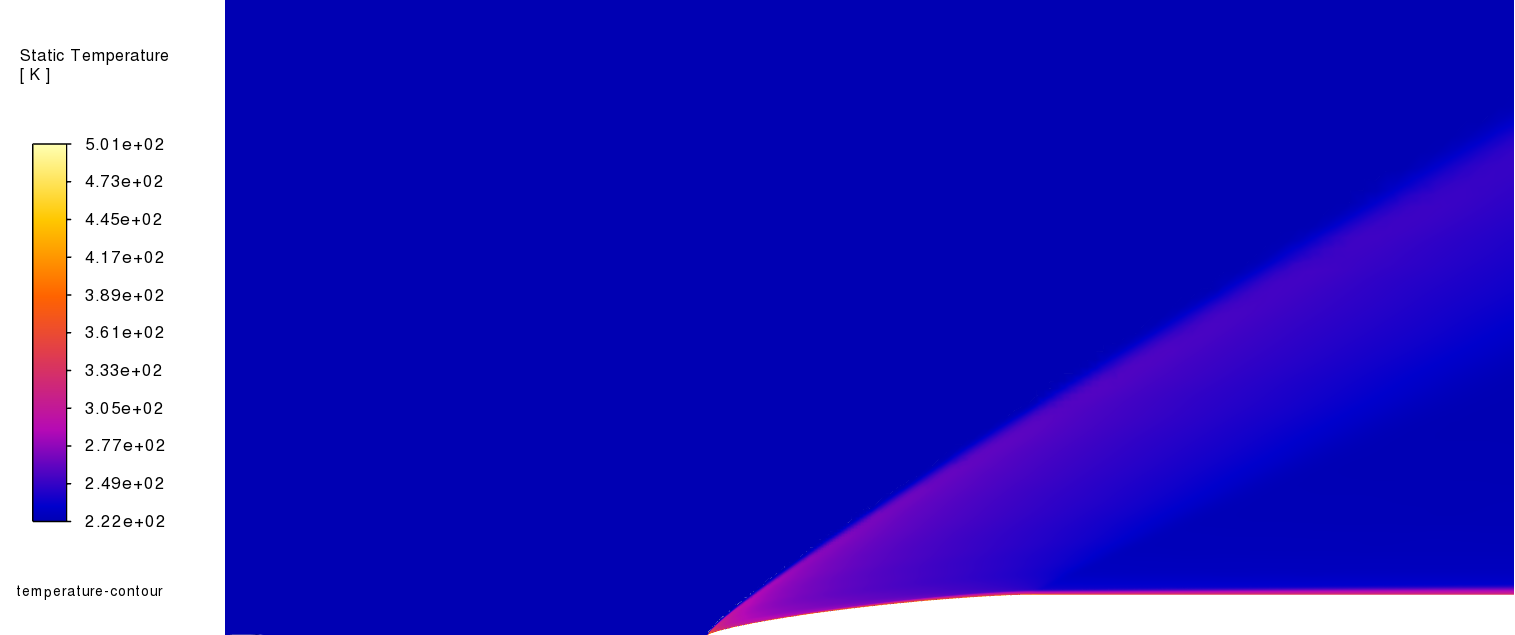
\includegraphics[height=0.23\textheight]{ansyspost/airflow/maxQ-temperature-contour.png}
        \caption{maxQ}
        \label{fig:maxQ_temp_contour}
    \end{subfigure}

    \begin{subfigure}{\textwidth}
        \centering
        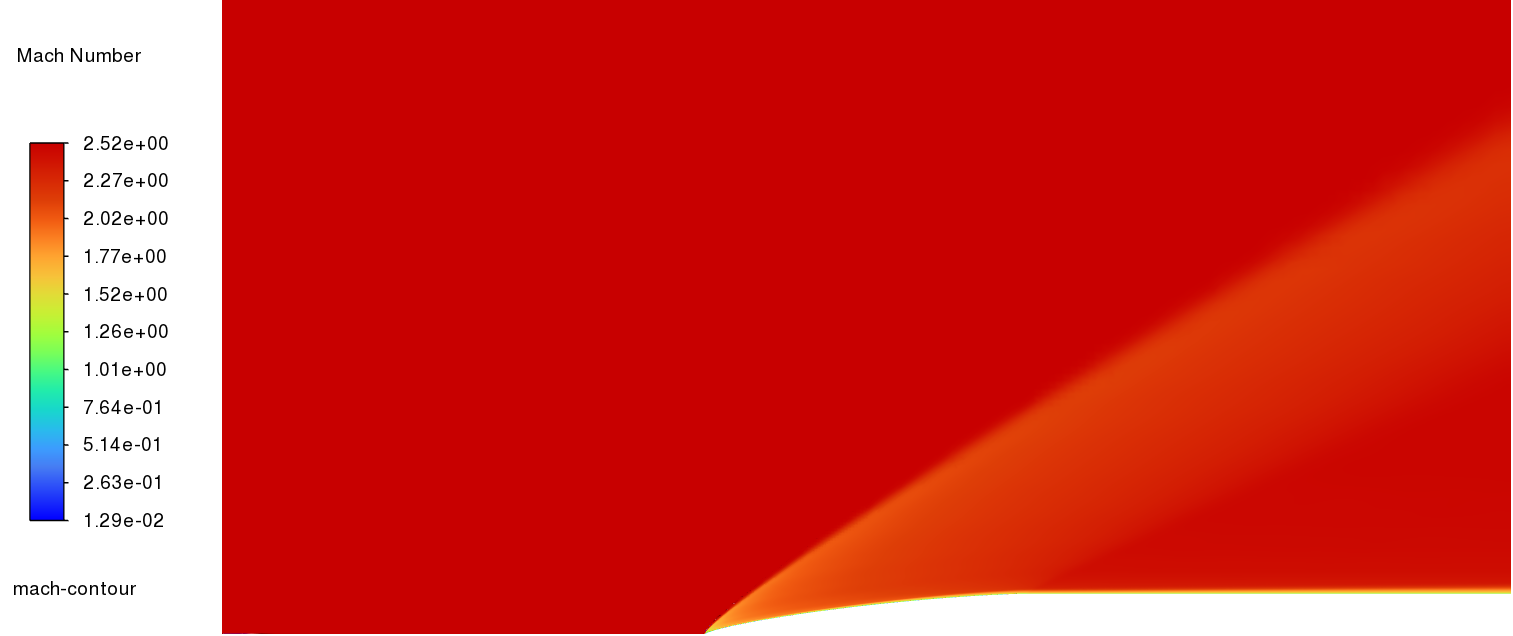
\includegraphics[height=0.23\textheight]{ansyspost/airflow/maxQ-mach-contour.png}
        \caption{maxQ}
        \label{fig:maxQ_mach_contour}
    \end{subfigure}

    \caption{max Q Konturen}
    \label{fig:maxQ_konturen}
\end{figure}


\subsection{\texorpdfstring{\ac{cht}}{CHT}}

\begin{figure}[H]
    \centering

    % Left figure
    \begin{minipage}{0.485\textwidth}
        \centering
        \setlength{\tabcolsep}{1pt} % reduce subfigure spacing
        \begin{subfigure}{0.24\textwidth}
            \centering
            
\includegraphics[height=0.7\textheight]{liquid-fraction-300.png}
            \caption{\SI{300}{\second}}
        \end{subfigure}%
        \begin{subfigure}{0.24\textwidth}
            \centering
            
\includegraphics[height=0.7\textheight]{liquid-fraction-600.png}
            \caption{\SI{600}{\second}}
        \end{subfigure}%
        \begin{subfigure}{0.24\textwidth}
            \centering
            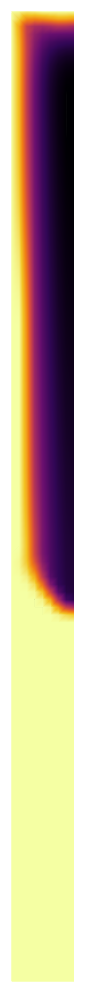
\includegraphics[height=0.7\textheight]{liquid-fraction-900.png}
            \caption{\SI{900}{\second}}
        \end{subfigure}%
        \begin{subfigure}{0.24\textwidth}
            \centering
            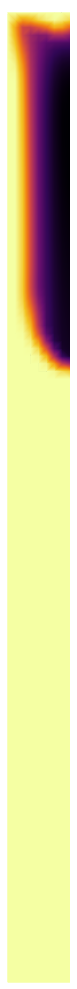
\includegraphics[height=0.7\textheight]{liquid-fraction-1200.png}
            \caption{\SI{1200}{\second}}
        \end{subfigure}
        \caption{Flüssigkeitsanteil Konturen}
        \label{fig:liquid_frac_contour}
    \end{minipage}
    \hspace{2mm} % small horizontal space
    % Right figure
    \begin{minipage}{0.485\textwidth}
        \centering
        \begin{subfigure}{0.24\textwidth}
            \centering
            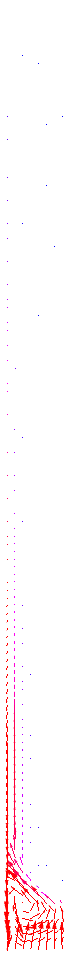
\includegraphics[height=0.7\textheight]{velocity-vector-300.png}
            \caption{\SI{300}{\second}}
        \end{subfigure}%
        \begin{subfigure}{0.24\textwidth}
            \centering
            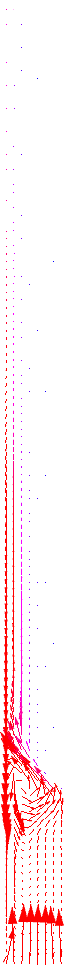
\includegraphics[height=0.7\textheight]{velocity-vector-600.png}
            \caption{\SI{600}{\second}}
        \end{subfigure}%
        \begin{subfigure}{0.24\textwidth}
            \centering
            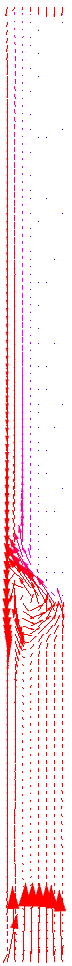
\includegraphics[height=0.7\textheight]{velocity-vector-900.png}
            \caption{\SI{900}{\second}}
        \end{subfigure}%
        \begin{subfigure}{0.24\textwidth}
            \centering
            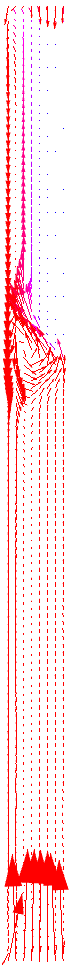
\includegraphics[height=0.7\textheight]{velocity-vector-1200.png}
            \caption{\SI{1200}{\second}}
        \end{subfigure}
        \caption{Geschwindigkeits-Vektoren nach Flüssigkeitsanteil gefärbt}
        \label{fig:velocity_vector}
    \end{minipage}

\end{figure}